\documentclass[11pt,a4paper]{ctexart}
\usepackage[margin=1.9cm]{geometry}
\usepackage{amsmath,amssymb,bm}
\usepackage{booktabs,graphicx,float,array,hyperref}
\hypersetup{colorlinks=true,linkcolor=blue,urlcolor=blue}
\setlength{\parindent}{2em}
\setlength{\parskip}{0.22em}
\title{原作者 IMU--UWB InEKF 的纯计算加速}
\author{算法、初值、偏置与噪声保持不变的直接对比}
\date{2026年7月24日}

\begin{document}
\maketitle
\pagestyle{plain}

\section{隔离目标}

本实验不比较算法改进，而是回答：在完整保留论文作者公开代码的状态、参数和更新
语义时，仅消除 Python 计算开销能获得多少加速。

原作者 backup 与加速目录中的 \texttt{inekf.py} 字节级相同：
\begin{equation}
\operatorname{SHA256}(\texttt{backup/inekf.py})
=
\operatorname{SHA256}(\texttt{acc/inekf.py})
=\texttt{97142a58\ldots cd6cb0c}.
\end{equation}
入口在每次运行前检查该等式；不成立则终止。

\section{完整保留的作者递推}

名义状态和误差协方差仍为
\begin{equation}
 X=(R,v,p)\in SE_2(3),\qquad P\in\mathbb R^{15\times15},
\end{equation}
并保留作者原始预测
\begin{align}
 R_{k+1}^{-}&=R_k^{+}\operatorname{Exp}
 ((\omega_k-b_{\omega})\Delta t),\\
 v_{k+1}^{-}&=v_k^{+}
 +[R_k^{+}(a_k-b_a)+g]\Delta t,\\
 p_{k+1}^{-}&=p_k^{+}+v_k^{+}\Delta t
 +\frac12[R_k^{+}(a_k-b_a)+g]\Delta t^2,\\
 P_{k+1}^{-}&=\Phi_kP_k^{+}\Phi_k^{\mathsf T}
 +\Phi_k\operatorname{Ad}_{X_{k+1}^{-}}
 Q_k\operatorname{Ad}_{X_{k+1}^{-}}^{\mathsf T}\Phi_k^{\mathsf T}.
\end{align}

TDoA 仍使用作者的左坐标预门限
\begin{equation}
 d_m^2=
 \frac{(y-h(X^-))^2}
 {H_lP^-H_l^{\mathsf T}+R},\qquad
 d_m\ge 5\ \Longrightarrow\ \text{reject},
\end{equation}
随后执行
\begin{align}
 H_r&=H_l\operatorname{Ad}_{(X^-)^{-1}},\\
 K&=P^-H_r^{\mathsf T}
 (H_rP^-H_r^{\mathsf T}+R)^{-1},\\
 P^+&=(I-KH_r)P^-(I-KH_r)^{\mathsf T}+KRK^{\mathsf T},\\
 X^+&=\operatorname{Exp}(-Kz)X^-.
\end{align}
原始偏置布局、零偏置初值、1 rad yaw 先验、0.13 TDoA 方差、地面钳位和
全部 IMU/UWB 调用均不改变。本实验也有意保留原作者已经识别的坐标和偏置问题。

\section{只改变计算映射}

原作者循环的执行成本可写为
\begin{equation}
 T_{\mathrm{Python}}
 =N(t_{\mathrm{dispatch}}+t_{\mathrm{allocation}}+t_{\mathrm{math}}).
\end{equation}
纯加速版在循环外生成事件整数索引和固定 float64 缓冲区，再把调度、预测和更新
一起编译为本机代码：
\begin{equation}
 T_{\mathrm{acc}}
 =T_{\mathrm{JIT,once}}+N\,t_{\mathrm{native}}.
\end{equation}

作者当前误差动力学的块结构满足
\begin{equation}
 A^4=0,
\end{equation}
因此通用矩阵指数可严格写为有限多项式
\begin{equation}
\boxed{
\Phi=e^{A\Delta t}
=I+A\Delta t+\frac12(A\Delta t)^2+\frac16(A\Delta t)^3
}.
\end{equation}
这不是截断近似。量测侧只把
$H_l\operatorname{Ad}_{(X^-)^{-1}}$ 直接展开，Joseph 更新仍完整保留。

\section{30 秒直接结果}

两边共享相同事件计划，正式计时排除数据加载、初始化、JIT、历史、指标和绘图，
并按 AB/BA 顺序交替四轮。每轮均处理 30,267 次预测和 14,289 次 UWB。

\begin{table}[H]
\centering
\caption{稳定态公平回放}
\begin{tabular}{lrrr}
\toprule
指标 & 作者原始版 & 纯计算加速版 & 结果\\
\midrule
中位数/s & 6.811990 & 0.216905 & 31.4054x\\
MAD/s & 0.062050 & 0.001329 & -\\
最小值/s & 6.734570 & 0.214860 & -\\
最大值/s & 6.884360 & 0.230287 & -\\
\bottomrule
\end{tabular}
\end{table}

首次无缓存 JIT 实测约 8.240 s；缓存加载/预热约 0.128 s，均没有计入表中。

\section{数值等价性}

\begin{table}[H]
\centering
\caption{作者原始版与纯计算加速版的最大绝对差}
\begin{tabular}{lr}
\toprule
量 & 最大绝对差\\
\midrule
旋转矩阵元素 & $6.77\times10^{-15}$\\
速度 & $5.54\times10^{-15}$ m/s\\
位置 & $3.33\times10^{-15}$ m\\
偏置 & $4.98\times10^{-19}$\\
NIS & $1.29\times10^{-14}$\\
UWB 拒绝决策变化 & 0\\
\bottomrule
\end{tabular}
\end{table}

位置、速度、姿态和 yaw RMSE 在显示精度内完全相同，两边 UWB 拒绝均为
$0/14289$。

\begin{figure}[H]
\centering
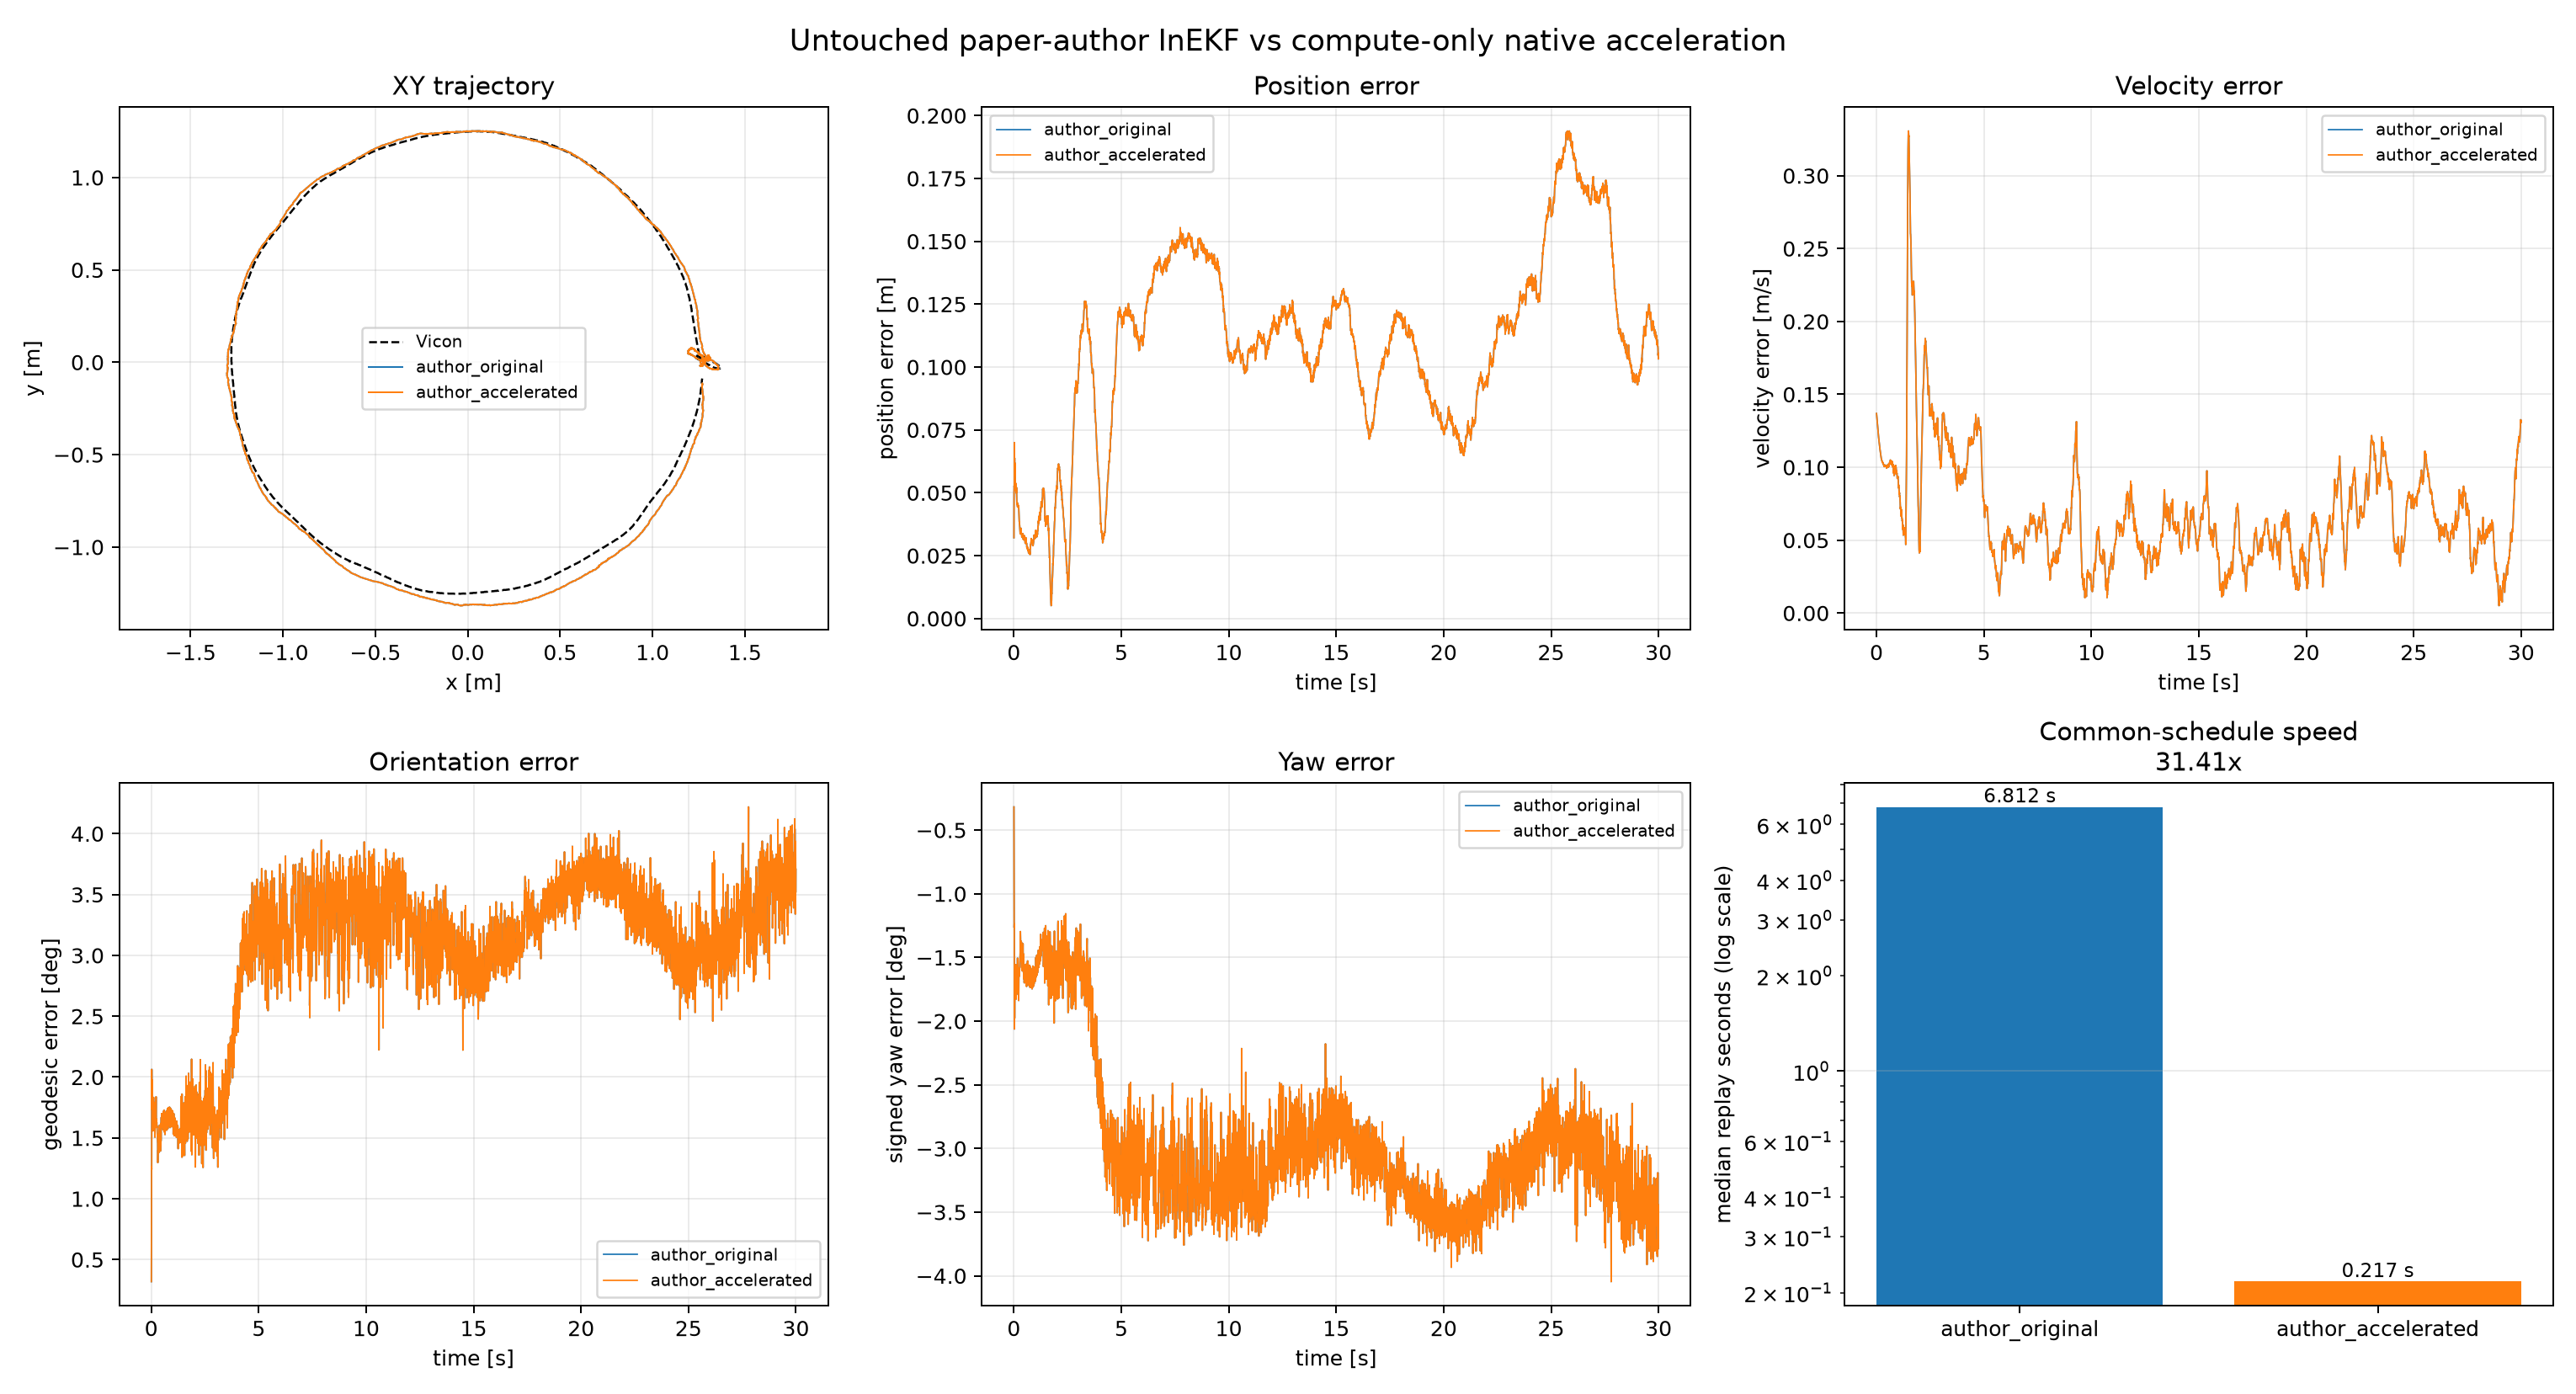
\includegraphics[width=0.92\textwidth]{../imu-uwb-inekf-acc/results/fair_author_original_vs_acc_const1_30s/comparison.png}
\caption{作者原始版与纯计算加速版：所有效果曲线逐点重合}
\end{figure}

\section{四个星座的完整代表文件}

进一步对四种锚点 constellation 各选择一个命名一致的代表文件并完整回放：
const1--const3 使用 trial1/TDoA2，const4 使用 trial1/TDoA2/traj1。每条均正式
重复两轮，不设置 \texttt{max-duration}。

\begin{table}[H]
\centering
\caption{完整文件单核回放中位数}
\begin{tabular}{lrrrr}
\toprule
数据 & 事件数 & 作者原始版/s & 纯计算加速版/s & 加速比\\
\midrule
const1 & 209426 & 45.645867 & 1.121883 & 40.6868x\\
const2 & 183197 & 39.344386 & 0.970576 & 40.5372x\\
const3 & 196615 & 43.110833 & 1.031722 & 41.7853x\\
const4 & 186075 & 40.473703 & 0.985142 & 41.0841x\\
\bottomrule
\end{tabular}
\end{table}

\begin{table}[H]
\centering
\caption{完整文件效果指标（两种实现显示精度内相同）}
\begin{tabular}{lrrrr}
\toprule
数据 & 位置 RMSE/m & 速度 RMSE/(m/s) & 姿态 RMSE/deg & yaw RMSE/deg\\
\midrule
const1 & 0.108003 & 0.060901 & 3.6570 & 3.5695\\
const2 & 0.103045 & 0.060616 & 1.6560 & 1.2562\\
const3 & 0.219516 & 0.167438 & 2.2330 & 2.0697\\
const4 & 0.200157 & 0.088926 & 3.2633 & 2.0724\\
\bottomrule
\end{tabular}
\end{table}

四组拒绝决策变化均为零；const1--const3 两边均无拒绝，const4 两边均拒绝同一条
UWB。最大状态差仍为 $10^{-14}$ 量级，最大 NIS 差不超过
$2.24\times10^{-13}$。

\begin{figure}[H]
\centering
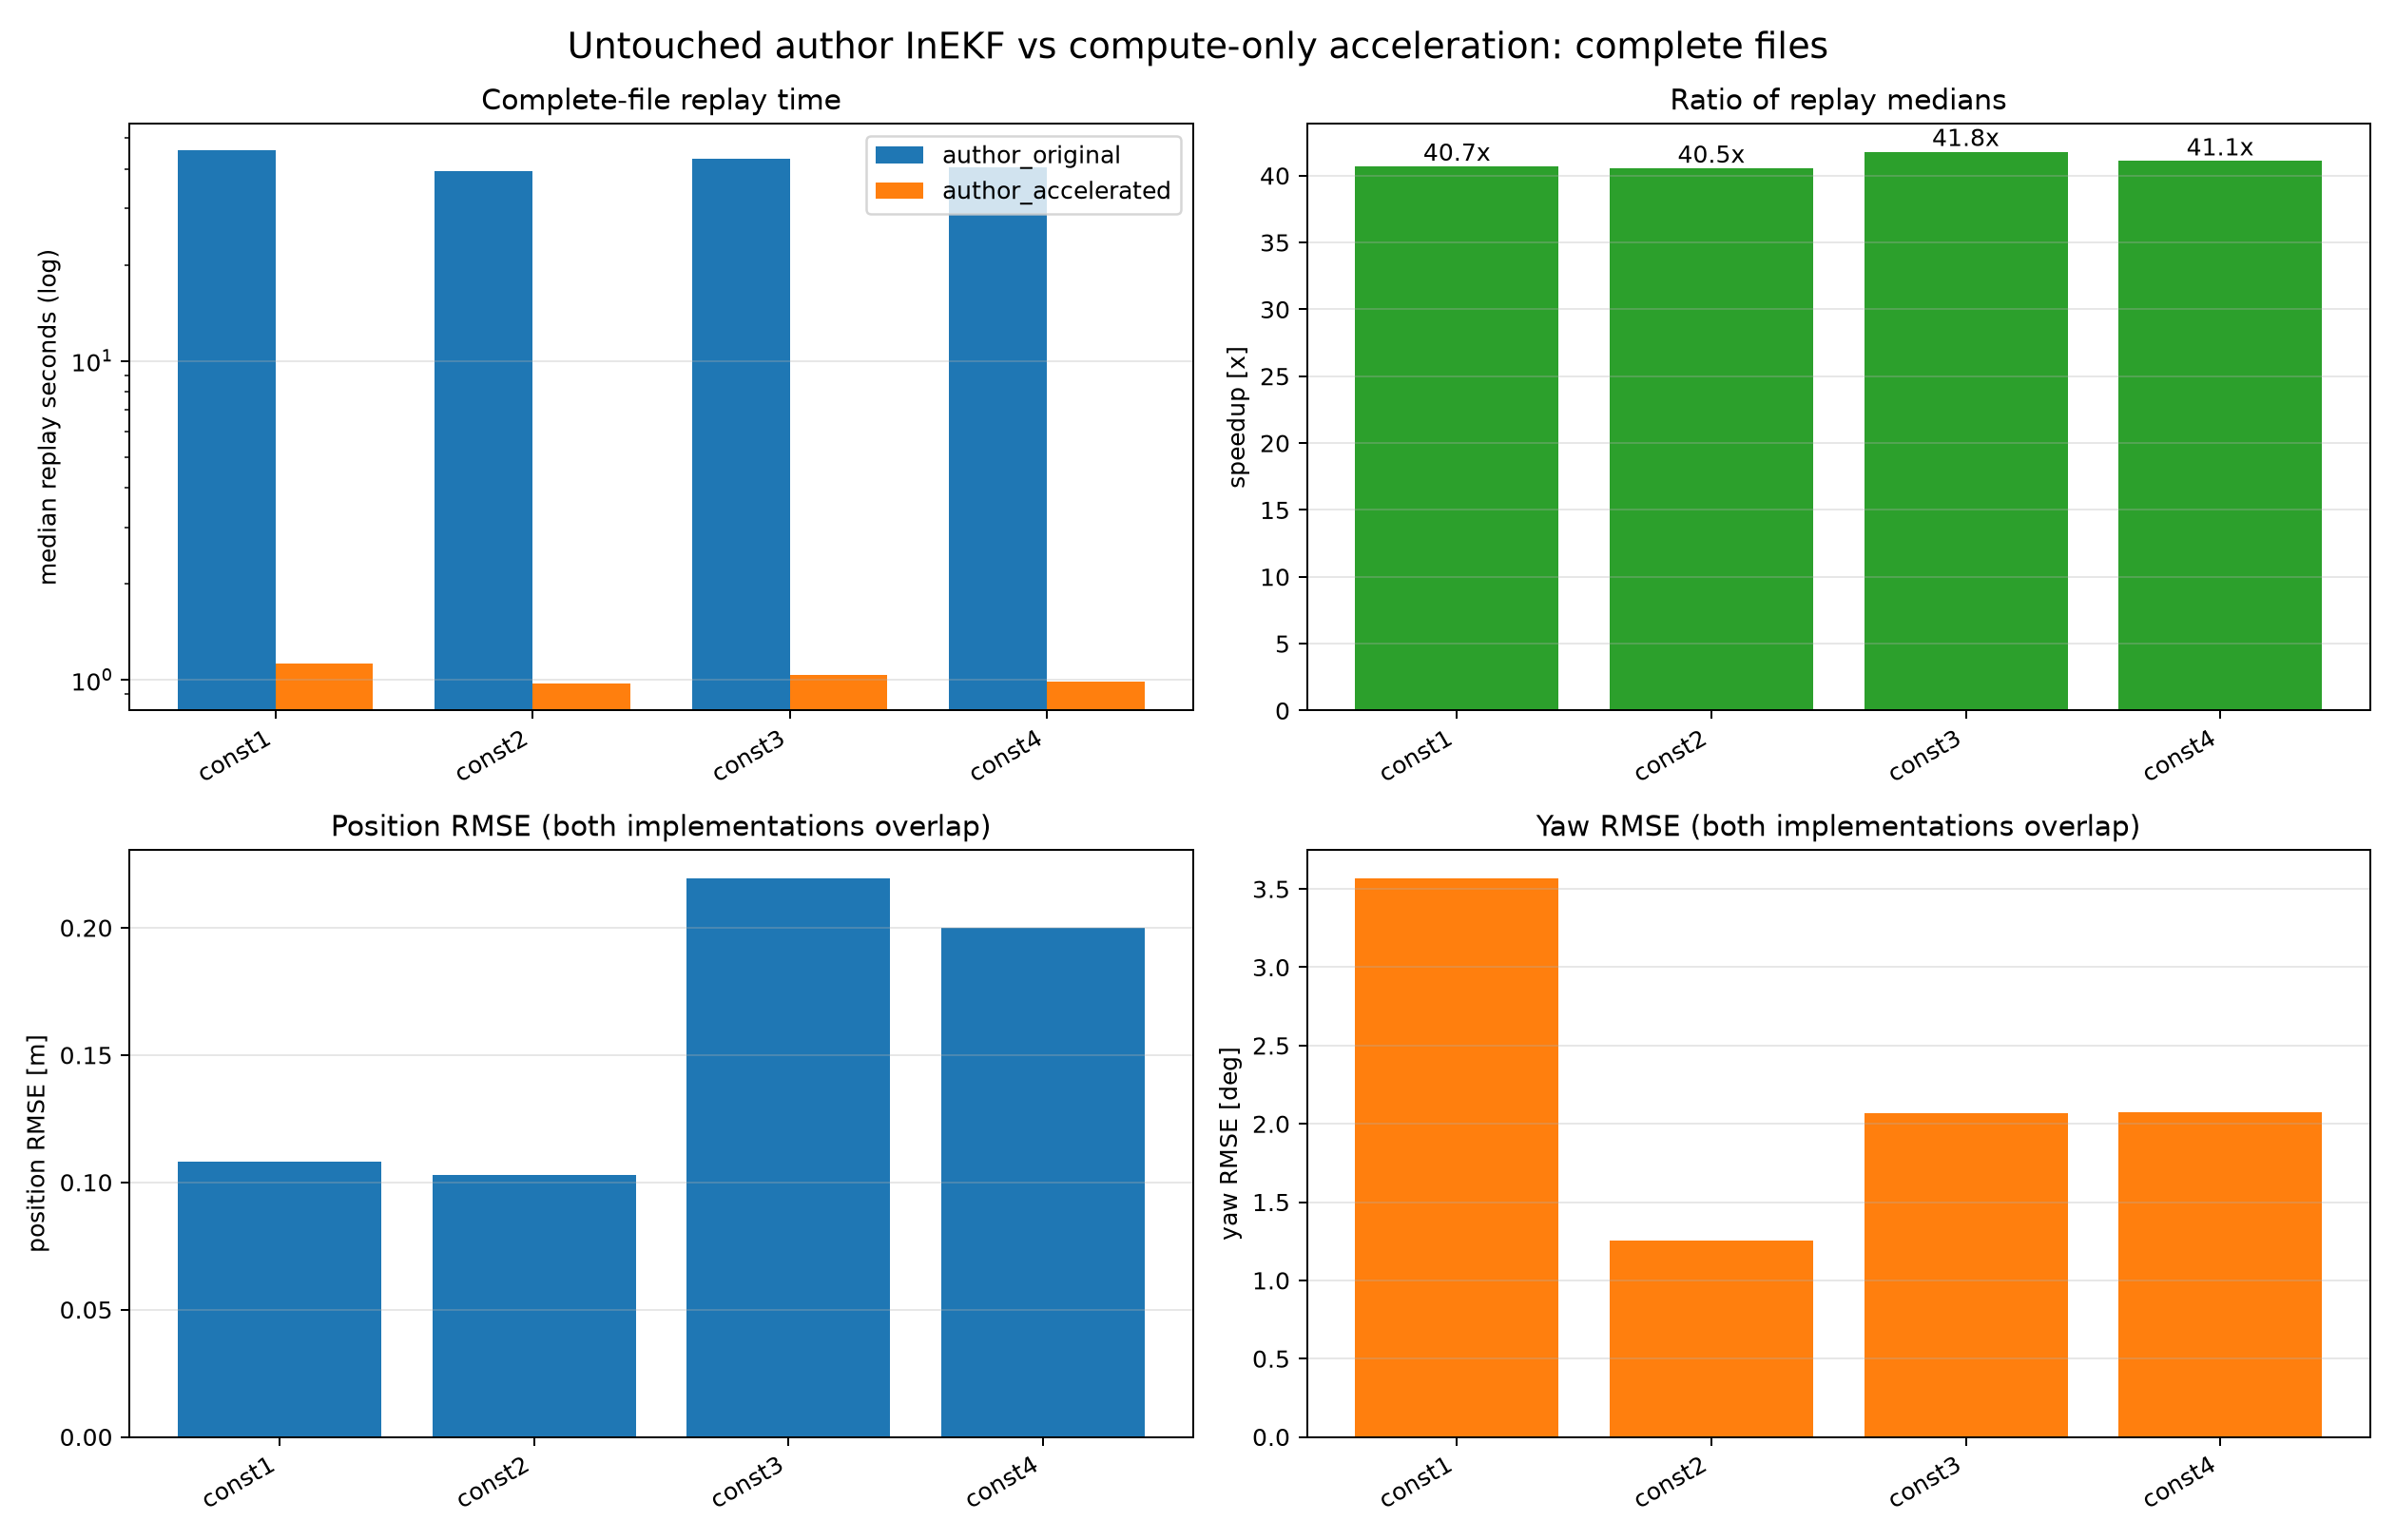
\includegraphics[width=0.96\textwidth]{../imu-uwb-inekf-acc/results/full_all_constellations/summary.png}
\caption{四个 constellation 完整代表文件的耗时与 RMSE 汇总}
\end{figure}

该批次为避免当前 Windows MKL 2026.1 与 LLVM OpenMP 的原生 DLL 冲突，固定
如下环境变量：
\begin{center}
\texttt{MKL\_THREADING\_LAYER=SEQUENTIAL}
\end{center}
因此表中的约 41 倍与前述旧运行库批次的 31.4 倍不能解释为算法再次加速；两者
均说明 Python 热循环消除后为数十倍量级。本节覆盖四个星座，但不是对数据集
全部 79 个 CSV 的穷举。

\section{20 核文件级并行穷举}

全部 79 个 CSV 彼此独立，适合在文件层并行；单条 CSV 内的滤波仍严格按时间
顺序执行，且每个子进程固定为 MKL 单线程并绑定一个逻辑 CPU。若工作进程 $j$
动态领取的文件集合为 $\mathcal A_j$，则
\begin{equation}
T_{\rm batch}(J)\approx
\max_{1\le j\le J}\sum_{i\in\mathcal A_j}T_i+T_{\rm overhead}.
\end{equation}
这只缩短离线批量总等待时间，不改变单条机载滤波延迟。

曲线回放不再保存未被指标或绘图消费的逐事件协方差历史。对于约 20 万事件，
\begin{equation}
M_{\rm covariance\ history}
=200000\times 15^2\times 8
\approx 360\ {\rm MB}.
\end{equation}
即每条文件约 360 MB。滤波内部仍逐事件传播完整 $15\times15$ 协方差；回归测试仍保存并逐项核对完整
协方差历史，故该变化不是降维、降频或算法近似。

\begin{table}[H]
\centering
\caption{四个完整文件同时运行的压力测试}
\begin{tabular}{lrrrr}
\toprule
数据 & 子进程墙钟/s & 作者中位数/s & 加速版中位数/s & 加速比\\
\midrule
const1 & 105.545 & 31.4105 & 0.9754 & 32.20x\\
const2 & 95.102 & 28.2619 & 0.8590 & 32.90x\\
const3 & 142.348 & 42.9766 & 1.0582 & 40.61x\\
const4 & 132.765 & 39.8653 & 0.9996 & 39.88x\\
\bottomrule
\end{tabular}
\end{table}

四条子进程墙钟之和为 475.760 s，批量墙钟为 142.353 s，即 3.342 倍调度收益
和 83.55\% 四核并行效率。观测峰值工作集约 1.06 GB；20 进程线性外推约
5.3 GB。四核实测吞吐理想外推 79 条约需 9.37 分钟；考虑异构核心、全核功耗、
绘图和磁盘开销，实际建议预留 12--20 分钟。

20 个固定核子进程同时运行 20 条短回放最终全部通过。该压力测试还发现一条
CSV 的首事件就是 UWB；旧调度器从第二个事件循环，会漏掉该量测。现已显式处理
初始 UWB 且不额外进行 IMU 预测，并以首事件含 UWB 的合成数据回归。修复后该
文件两边均执行 2017 次预测、573 次 UWB，拒绝决策相同，RMSE 一致。

完整入口使用
\begin{center}
\texttt{--all-files --jobs 20 --cpu-list 0-19 --repeats 2}\\
\texttt{--warmup-duration 10 --resume}
\end{center}
且不传 \texttt{max-duration} 或 \texttt{limit-cases}。并发绝对计时反映加载
系统吞吐；论文中的单核绝对速度仍应在空闲系统以 \texttt{--jobs 1} 复测。

\section{全部 79 个完整文件的最终验证}

全部 CSV 已实际完成，不是抽样或外推。共有 79 个文件、13,548,996 个事件、
9,984,576 次 IMU 预测和 3,564,341 次 UWB 更新。结果如下：
\begin{table}[H]
\centering
\caption{79 个完整文件的全量统计}
\begin{tabular}{lr}
\toprule
指标 & 结果\\
\midrule
成功/失败 & 79/0\\
加速比中位数 & 38.9794x\\
加速比范围 & 31.0226x--47.9746x\\
加速比四分位区间 & 32.8972x--41.2012x\\
作者中位耗时之和 & 2798.184 s\\
加速中位耗时之和 & 73.485 s\\
时间之和的比值 & 38.0781x\\
UWB 拒绝（作者/加速） & 17178/17178\\
拒绝决策变化 & 0\\
\bottomrule
\end{tabular}
\end{table}

\begin{table}[H]
\centering
\caption{各 constellation 的效果分布与速度}
\begin{tabular}{lrrrr}
\toprule
数据 & 文件数 & 加速比中位数 & 位置 RMSE 中位/最大 m & yaw RMSE 中位/最大 deg\\
\midrule
const1 & 12 & 36.7920x & 0.1136/0.1292 & 3.9866/5.6160\\
const2 & 12 & 39.2129x & 0.1059/0.1236 & 1.4431/3.9568\\
const3 & 16 & 39.1893x & 0.1851/0.3117 & 1.6051/3.9312\\
const4 & 39 & 38.3087x & 0.4285/0.8882 & 3.1738/10.6238\\
\bottomrule
\end{tabular}
\end{table}

最大旋转、速度、位置、偏置和 NIS 差分别为
$3.33\times10^{-14}$、$4.84\times10^{-14}$、
$3.80\times10^{-14}$、$9.85\times10^{-18}$ 和
$8.27\times10^{-9}$；最大 RMSE 绝对差不超过 $6.05\times10^{-15}$。
这些舍入差没有改变任何 UWB 决策。

const4 的位置和 yaw 分布明显较宽，但最差条目的作者/加速曲线仍逐点重合，说明
它是作者算法与数据组合的既有表现，而不是计算加速退化。全部 79 组曲线、指标
和日志均完整；总览图以及速度、位置、姿态、yaw 和 NIS 极值条目已经目检。
从首条 case 日志到汇总完成的端到端墙钟为 11.41 分钟，其中包含一次前台监控
连接中断及 \texttt{resume} 无损续跑。

\section{解释边界}

$31.4$ 倍是当前 Windows/Conda/单线程离线 Python 回放的直接结果，不是机载
WCET。其主要收益是消除 Python 热循环；若双方都实现为优化 C/C++，该倍数不会
自动保留。首次 JIT、部署依赖、编译核调试和双实现维护是主要工程代价。
此外，本目录为隔离变量而保留原作者算法问题，只能用于计算开销研究，不能替代
当前已修复的生产 InEKF。

\end{document}
